\section{Simulated-Annealing-Methode}

\begin{frame}
  \frametitle{Grundidee}
  \begin{itemize}
    \item Zerlegung $N=A\cdot B$ mit $B \leq A$
    \pause{}
    \item $A$, $B$ und $N$ werden als binäre Zahlen dargestellt
    \pause{}
    \item $a$, $b$ und $n$ sind die Längen der Zahlen ($\lc\log_2 A\rc$ usw.)
    \pause{}
    \item $a_1$ und $b_1$ sind die Zahlen der $1$en
      \begin{align*}
        2 \leq a \leq n \quad&\quad 1 \leq a_1 \leq a \\
        2 \leq b \leq a \quad&\quad	1 \leq b_1 \leq b
      \end{align*}
    \pause{}
    \item Der Suchbereich kann eingeschränkt werden (ca. $16\%$)
      \begin{align*}
        a_{\min}&=\begin{cases} 2 & \mathrm{falls}\;\; \lf\frac{n}{2}\rf=1 \\ \lf\frac{n}{2}\rf & \mathrm{sonst} \end{cases} \\
        b_{\min}&=\begin{cases} 2 & \mathrm{falls}\;\; n-a=1 \\ n-a & \mathrm{sonst} \end{cases}
      \end{align*}
  \end{itemize}
\end{frame}

\begin{frame}
  \frametitle{Vorgehen}
  \begin{enumerate}
    \item Einführung einer Energiedefinition
    \pause{}
    \item Operationen zur Modifikation des Zustandes
    \pause{}
    \item Algorithmus zur Akzeptanz oder Zurückweisung des neuen Zustandes (Metropolis)
    \pause{}
    \item Prüfung ob der Zustand eine Lösung ist
  \end{enumerate}
\end{frame}

\begin{frame}
  \frametitle{Energiedefinition}
  Es wird eine Energiedefinition eingeführt:
  \begin{equation*}
    E\left(A,B,N\right)=\sum\limits_{i=1}^N\begin{cases}f\left(i\right) & \mathrm{falls} {\left\{A\cdot B\right\}}_i={\left\{N\right\}}_i \\ 0 & \mathrm{sonst}\end{cases}
  \end{equation*}
  \pause{}
  $f\left(i\right)$ ist eine monoton steigende Funktion. \\
  \Rightarrow{} Übereinstimmung von $A\cdot B$ mit $N$ erhöht die Energie \\
  \Rightarrow{} Energie maximieren
  \pause{}
  \begin{align*}
    f\left(i\right)=i \quad&\Rightarrow\quad E_\mathrm{\max}\left(n\right)=\frac{n\left(n+1\right)}{2} \\
    f\left(i\right)=i^2 \quad&\Rightarrow\quad E_\mathrm{\max}\left(n\right)=\frac{n\left(n+1\right)\left(2n+1\right)}{6}\text{~\cite{oeis}}
  \end{align*}
\end{frame}

\begin{frame}
  \frametitle{Operationen}
  \begin{itemize}
    \setlength{\itemsep}{5pt}
    \item\textbf{Swap:} Tausche zwei zufällige Bits mit unterschiedlichem Wert
      \begin{figure}[H]
        \centering
        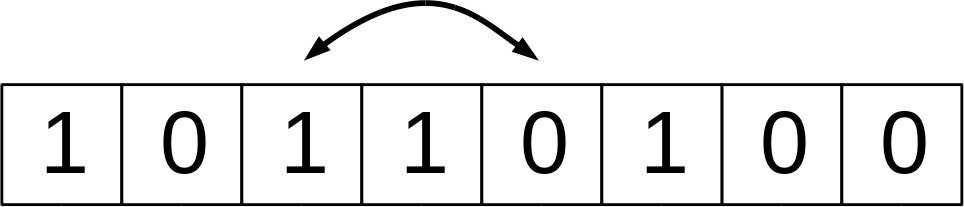
\includegraphics[width=3cm]{fig/bits-swap.png}
      \end{figure}
      \pause{}
    \item\textbf{Reverse:} Zufällige Bitsequenz umkehren
      \begin{figure}[H]
        \centering
        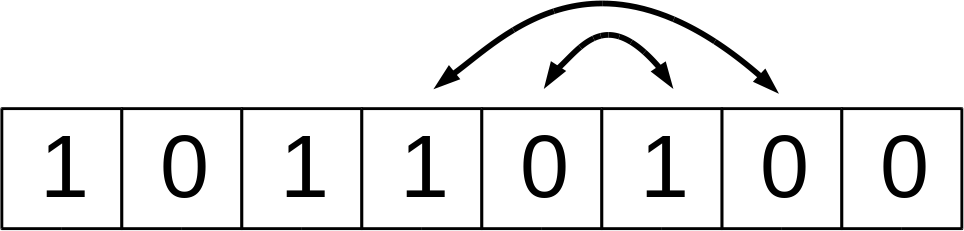
\includegraphics[width=3cm]{fig/bits-reverse.png}
      \end{figure}
      \pause{}
    \item\textbf{Slide:} Es wird eine zufällige Bitsequenz nach rechts geschoben
      \begin{figure}[H]
        \centering
        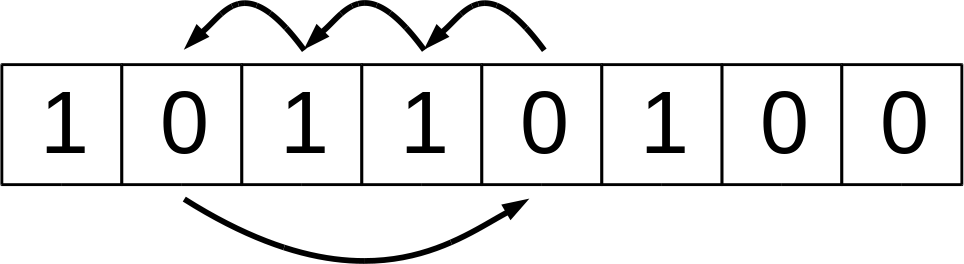
\includegraphics[width=3cm]{fig/bits-slide.png}
      \end{figure}
      \pause{}
    \item\textbf{Shuffle:} Bits zufällig auswählen und permutieren
  \end{itemize}
  Operationen haben Laufzeit $\mathcal{O}\left(n\right)$
\end{frame}

\begin{frame}
  \frametitle{Metropolis-Algorithmus}
  \begin{algorithmic}[1]
  \small
  \Procedure{Metropolis}{$A,B,E,N$}
    \If{$\mathrm{randomInt}\left(0,1\right) = 0$}
      \State{$A^\prime\gets\mathrm{randomOperation}\left(A\right)$}
    \Else{}
      \State{$B^\prime\gets\mathrm{randomOperation}\left(B\right)$}
    \EndIf{}
    \If{$A\cdot B=N$}
      \State{Exit}\Comment{Faktoren $A, B$ wurden gefunden}
    \EndIf{}
    \State{$E^\prime=E\left(A^\prime,B^\prime,N\right)$}
    \If{$E^\prime>E$}
      \State{$A\gets A^\prime$, $B\gets B^\prime$, $E\gets E^\prime$}
    \Else{}
      \State{$p\gets\mathrm{randomFloat}\left(0.0, 1.0\right)$}
      \If{$p<\exp\left(-\frac{E^\prime-E}{k_\mathrm{B} T}\right)$}
        \State{$A\gets A^\prime$, $B\gets B^\prime$, $E\gets E^\prime$}
      \EndIf{}
    \EndIf{}
  \EndProcedure{}
  \normalsize
\end{algorithmic}

\end{frame}

\begin{frame}
  \frametitle{Annealing-Algorithmus}
  Parameter:
  \begin{itemize}
    \item $N_a$: Anzahl der Abkühlungsschritte
    \item $N_c$: Anzahl der Konfigurationen pro Abkühlungsschritt
    \item $F_c$: Abkühlungsfaktor
  \end{itemize}
  \vspace{0.5cm}
  \begin{algorithmic}[1]
  \Procedure{Anneal}{$A,B,E,N$}
    \State{$T\gets 1.0$}
    \For{$i\gets 1$ to $N_a$}
      \For{$j\gets 1$ to $N_c$}
        \State{$\mathrm{Metropolis}\left(A,B,E,N\right)$}
      \EndFor{}
      \State{$T\gets T\cdot F_c$}
    \EndFor{}
  \EndProcedure{}
\end{algorithmic}

\end{frame}

\begin{frame}
  \frametitle{Zerlegungsschritt}
  \begin{algorithmic}[1]
  \small
  \Procedure{Factorize}{$N$}
    \State{$a_\mathrm{min}$ berechnen}
    \For{$a\in\left[a_\mathrm{min}, n\right]$}
      \For{$a_1\in\left[1,a\right]$}
        \State{$A\gets\mathrm{randomBitset}\left(a, a_1\right)$}
        \State{$b_\mathrm{min}$ berechnen}
        \For{$b\in\left[b_\mathrm{min}, a\right]$}
          \For{$b_1\in\left[1,b\right]$}
            \State{$B\gets\mathrm{randomBitset}\left(b, b_1\right)$}
            \State{$E\gets E\left(A,B,E,N\right)$}
            \If{$A\cdot B=N$}
              \State{Exit}\Comment{Faktoren $A, B$ wurden gefunden}
            \EndIf{}
            \State{$\mathrm{anneal}\left(A,B,E,N\right)$}
          \EndFor{}
        \EndFor{}
      \EndFor{}
    \EndFor{}
  \EndProcedure{}
  \normalsize
\end{algorithmic}

\end{frame}

\begin{frame}[allowframebreaks]
  \frametitle{Abschätzung der Laufzeit}
  Abschätzung der Worst-Case-Laufzeit:
  \begin{itemize}
    \item Annealing-Algorithmus wird $\mathcal{O}\left(n^4\right)$-mal ausgeführt (Wertebereiche von $a$, $b$, $a_1$ und $b_1$ skalieren grob mit $\mathcal{O}\left(n\right)$)
    \item dabei wird der Metropolis-Algorithmus $\mathcal{O}\left(N_a\cdot N_c\right)$-mal ausgeführt
    \item dort jeweils eine der $4$ Operationen mit Laufzeit $\mathcal{O}\left(n\right)$
  \end{itemize}
  \Rightarrow{} Laufzeit eines Zerlegungsschrittes $\mathcal{O}\left(n^5\cdot N_a\cdot N_c\right)$
  \pause{}
  \begin{figure}[H]
    \centering
    \includegraphics[width=\textwidth,height=0.8\textheight,keepaspectratio]{plot/runtime-sieve/plot.pdf}
  \end{figure}
\end{frame}
